\providecommand{\main}{..}
\documentclass[../mthe-493-final-project.tex]{subfiles}

% Overall implementation of our design solution.
\begin{document}
    \chapter{Implementation}
    \label{ch:implementation}

    \section{Optimization}
    \label{sec:optimization-implementation}

    % \subsection{Data Allocation Optimization}
    % \label{ssec:data-allocation-optimization}
    % % Algorithm implementation. Includes all tested algos and which was selected and why. Visualizes algo's approach to the optimum. Describes code implementation.

    % \subsubsection{Qualifying Assumptions}
    % The system is designed so that the following assumptions are met to ensure the feasibility of a solution to the optimization problem.

    % \begin{enumerate}
    %     \item $k \geq \beta$ where $\beta$ is set as the minimum amount of workers to be distributed to.
    %     \item $n \geq s^{min} \cdot k$
    %     \item $s_i^{max} \geq s^{min}$ for $i = 1,..,k$
    %     \item $n \leq \sum_{i=1}^k s_i$, ensuring there is enough combined compute capacity to accept the entire data set.

    % \end{enumerate}

    % \subsubsection{Implementation}

    % As discussed in the midterm presentation, multiple ILP algorithms will be researched, implemented, tested, and evaluated. A preliminary list of algorithms includes

    % \begin{enumerate}
    %     \item LP relaxation of the ILP problem (e.g., simplex, dual simplex)
    %     \item Branch and cut method with LP (e.g., simplex, dual simplex)
    %     \item Hill climbing technique
    % \end{enumerate}

    % \subsubsection{Heuristic Algorithm}
    % The following is a heuristic algorithm for achieving an optimal solution to the problem.

    % \textbf{Assumptions without loss of generality}
    % \begin{enumerate}
    %     \item $s_i^{max}$, $s_{min}$, $n$, and $k$ are nonnegative integers.
    %     \item $0 \leq c_1 \leq c_2 \leq ... \leq c_k$ Otherwise rearrange the terms.
    % \end{enumerate}

    % \textbf{Procedure}
    % \begin{enumerate}
    %     \item If \[ \sum_{i=1}^k s_i = n, \] then $x_i = s_i$, $i = 1,...,k$ is the optimal solution.
    %     \item If \[\sum_{i=1}^k s_i > n,\] then let $x_i = s^{min}$ for $i = 1,...,k$.
    %     \item Set $l = 1$. Add 1 to $x_l$ until $x_l = s_l^{max}$, then let $l = l+1$ and repeat. Continue until \[ \sum_{i=1}^{k} x_i = n \]. This yields the optimal solution.
    % \end{enumerate}

    \section{Distributed Computing}
    \label{sec:distributed-computing-implementation}

    % "Performs an economic analysis on multiple solutions and uses quantitative justification when choosing solution"
    %
    % Buting compute credits from KDS vs using AXON for "free". i.e., energy costs

    \subsection{Cycle Time \& Benchmarks}
    \label{ssec:cycle-time-and-benchmarks}

    \todo{Need to make this section more formal, and include proper citations to Duncan's work.}

    As specified by Duncan's work, each worker $w_i$ will be benchmarked to estimate

    \begin{enumerate}
        \item an \textit{upload/download rate}, $b_i$
        \item a \textit{sample compute rate}, $C_i$
    \end{enumerate}

    Each worker also has a \textit{fee} to compute a sample, $c_i$. Together, we can define the following quantities:

    \begin{itemize}
        \item \textit{Subjob download time}, $t^d_i$, which is a function of $s_i$
              \[t^d_i = \frac{P_m + P_d s_i}{b_i}\]
        \item \textit{Subjob compute time}, $t^c_i$, which is a function of $s_i$
              \[t^c_i = \frac{\tau s_i}{C_i}\]
        \item \textit{Subjob upload time}, $t^u_i$, which is fixed for a given job
              \[t^u_i = \frac{P_m}{b_i}\]
    \end{itemize}

    A worker's \textit{global cycle time} to compute a subjob is

    \[t_i = t^d_i + t^c_i + t^u_i\]

    The upper bound on training time yields an inequality

    \[t_i < T \quad \forall w_i \in \mathbf{W}\]

    from which an upper bound on \textit{subjob size} is derived

    \[s^{max}_i < \frac{T - \frac{2 P_m}{b_i}}{\frac{\tau}{C_i} - \frac{P_d}{b_i}}\]

    Note that these details are internal to Duncan's research and implementation. We intend to use this implementation to determine $s^{max}_i$.

    \subsection{Network Implementation}
    \label{ssec:network-implementation}
    %Description of approach and final code-base architecture. Our physical model. Great place for an architecture diagram.
    % Naive translation form math model to actual implementation.
    % e.g., workers are represented as machines on a network

    \begin{figure}
        \centering
        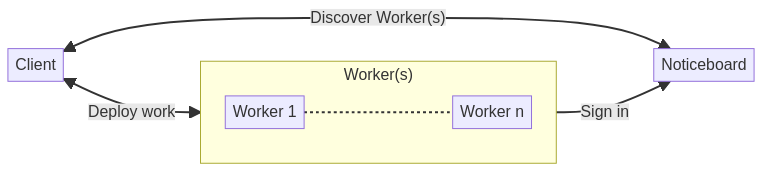
\includegraphics{network-1.png}
        \caption{Caption}
        \label{fig:network-flowchart}
    \end{figure}

    \begin{figure}
        \centering
        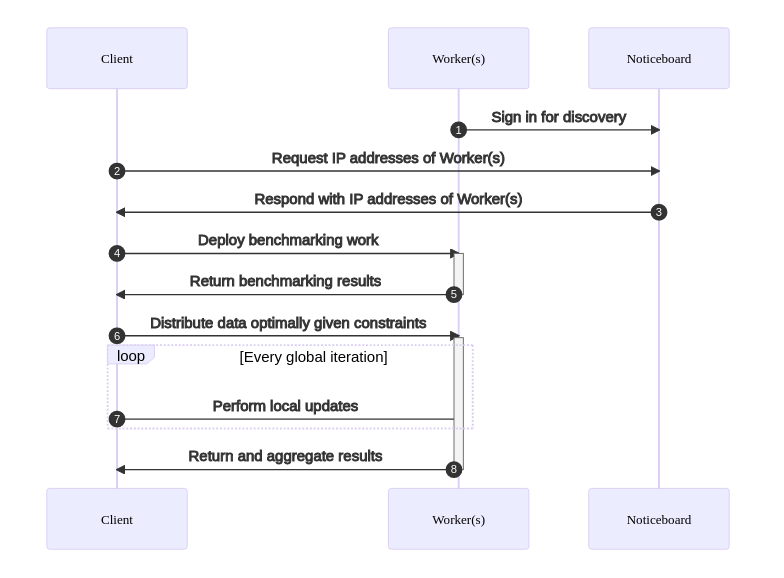
\includegraphics{network-2.png}
        \caption{Caption}
        \label{fig:network-sequence}
    \end{figure}

    \section{Federated Learning}
    \label{sec:federate-learning}
\end{document}
